%
%===============>>  Гусев Модуль 8 <<=============
%
\setmodule{8}

%BEGIN_FOLD % ====>>_____ Занятие 1 _____<<====
\begin{class}[number=1]
	\begin{listofex}
		\item
		\begin{minipage}[t]{\bodywidth}
			Определите координаты точек:
		\end{minipage}
		%\hspace{0.02\linewidth}
		\begin{minipage}[c]{0.45\textwidth}
			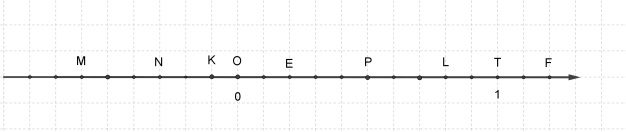
\includegraphics[align=t, width=\linewidth]{../\picpath/G61M6L1-1}
		\end{minipage}
	\end{listofex}
\begin{definit}
Чтобы вычесть из отрицательного числа отрицательное число, нужно сложить их так, будто они положительные, а перед суммой поставить минус.
\end{definit}
\begin{listofex}[resume]
\item Вычислите:
\begin{tasks}(4)
	\task \( -28-14 \)
	\task \( -144-56 \)
	\task \( -9-17 \)
	\task \( -3-18 \)
	\task \( -12-7 \)
	\task \( -15-8 \)
	\task \( -24-19 \)
	\task \( -8-3 \)
\end{tasks}
\end{listofex}
\begin{definit}
Для удобства, при сложении отрицательного числа с положительным, сумму можно записать как разность, поставив положительное число перед отрицательным. \\ Например, \(-12+25=25-12=13\).
\end{definit}
\begin{listofex}[resume]
\item Вычислите:
\begin{tasks}(4)
	\task \( -35 + 92 \)
	\task \( -7+14 \)
	\task \( -17+21 \)
	\task \( -5+65 \)
	\task \( -26+27 \)
	\task \( -8+12 \)
	\task \( -32+32 \)
	\task \( -80+124 \)
\end{tasks}
\end{listofex}
\begin{definit}
Если перед скобками стоит знак минус, то при их раскрытии знак внутри скобок меняется на противоположный. \\ Например: \(-(-a) = a \) или \( -(b) = -b \)
\end{definit}
\begin{listofex}[resume]
\item Вычислите:
\begin{tasks}(3)
	\task \( -35 - (-42) \)
	\task \( 8-(6) \)
	\task \( -(19)-(-21) \)
	\task \( -5-(-27) \)
	\task \( -(-42)+18 \)
	\task \( -(-17)-26 \)
	\task \( -(-29)+(-13) \)
	\task \( -(18)+(-12) \)
\end{tasks}
\end{listofex}
\begin{definit}
Чтобы из меньшего числа вычесть большее, необходимо из большего вычесть меньшее и перед результатом поставить знак минус. \\ Например: \( 17-82 = -(82-17)=-65 \)
\end{definit}
\begin{listofex}[resume]
\item Вычислите:
\begin{tasks}(4)
	\task \( 15-21 \)
	\task \( 17-66 \)
	\task \( 100-143 \)
	\task \( 42-69 \)
	\task \( 85-98 \)
	\task \( 117-162 \)
	\task \( 31-67 \)
	\task \( 71-143 \)
\end{tasks}
	\end{listofex}
\end{class}
%END_FOLD

%BEGIN_FOLD % ====>>_____ Занятие 2 _____<<====
\begin{class}[number=2]
	\begin{listofex}
		\item Занятие 2
	\end{listofex}
\end{class}
%END_FOLD

%BEGIN_FOLD % ====>>_ Домашняя работа 1 _<<====
\begin{homework}[number=1]
	\begin{listofex}
		\item
		\begin{minipage}[t]{\bodywidth}
			Определите координаты всех точек:
		\end{minipage}
		%\hspace{0.02\linewidth}
		\begin{minipage}[c]{0.7\linewidth}
			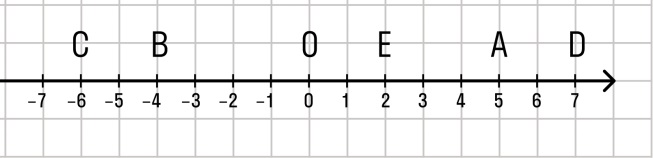
\includegraphics[align=t, width=\linewidth]{../\picpath/G61M6L2-1}
		\end{minipage}
		\item Вычислите:
		\begin{tasks}(2)
		\task \( -11 + 21 \)
		\task \( -17+25 \)
		\task \( -37+65 \)
		\task \( -51-14 \)
		\task \( -26-37 \)
		\task \( -83-22 \)
		\end{tasks}
		\item В четырех домах \(567\) жителя. В одном доме \(\dfrac{1}{3}\) всех жителей, во втором --- в \(1,5\) раза меньше, чем в первом, а остальные живут поровну в третьем и четвёртом домах. По скольку жителей живёт в третьем и четвёртом домах?
	\end{listofex}
\end{homework}
%END_FOLD

%BEGIN_FOLD % ====>>_____ Занятие 3 _____<<====
\begin{class}[number=3]
	\begin{listofex}
		\item Занятие 3 
	\end{listofex}
\end{class}
%END_FOLD

%BEGIN_FOLD % ====>>_____ Занятие 4 _____<<====
\begin{class}[number=4]
	\begin{listofex}
		\item Занятие 4
	\end{listofex}
\end{class}
%END_FOLD

%BEGIN_FOLD % ====>>_ Домашняя работа 2 _<<====
\begin{homework}[number=2]
	\begin{listofex}
		\item Домашняя работа 2
	\end{listofex}
\end{homework}
%END_FOLD

%BEGIN_FOLD % ====>>_____ Занятие 5 _____<<====
\begin{class}[number=5]
	\begin{listofex}
		\item Занятие 5
	\end{listofex}
\end{class}
%END_FOLD

%BEGIN_FOLD % ====>>_____ Занятие 6 _____<<====
\begin{class}[number=6]
	\begin{listofex}
		\item Занятие 6
	\end{listofex}
\end{class}
%END_FOLD

%BEGIN_FOLD % ====>>_ Домашняя работа 3 _<<====
\begin{homework}[number=3]
	\begin{listofex}
		\item Домашняя работа 3
	\end{listofex}
\end{homework}
%END_FOLD

%BEGIN_FOLD % ====>>_____ Занятие 7 _____<<====
\begin{class}[number=7]
	\title{Подготовка к проверочной}
	\begin{listofex}
		\item Занятие 7
	\end{listofex}
\end{class}
%END_FOLD

%BEGIN_FOLD % ====>>_ Проверочная работа _<<====
\begin{exam}
	\begin{listofex}
		\item Проверочная
	\end{listofex}
\end{exam}
%END_FOLD